\documentclass[12pt]{report}
\usepackage[utf8]{inputenc}
\usepackage[russian]{babel}
%\usepackage[14pt]{extsizes}
\usepackage{listings}
\usepackage{graphicx}
\usepackage{amsmath,amsfonts,amssymb,amsthm,mathtools} 
\usepackage{pgfplots}
\usepackage{filecontents}
\usepackage{float}
\usepackage{comment}
\usepackage{indentfirst}
\usepackage{eucal}
\usepackage{enumitem}
%s\documentclass[openany]{book}
\frenchspacing

\usepackage{indentfirst} % Красная строка

\usetikzlibrary{datavisualization}
\usetikzlibrary{datavisualization.formats.functions}

\usepackage{amsmath}


% Для листинга кода:
\lstset{ %
	language=c,                 % выбор языка для подсветки (здесь это С)
	basicstyle=\small\sffamily, % размер и начертание шрифта для подсветки кода
	numbers=left,               % где поставить нумерацию строк (слева\справа)
	numberstyle=\tiny,           % размер шрифта для номеров строк
	stepnumber=1,                   % размер шага между двумя номерами строк
	numbersep=5pt,                % как далеко отстоят номера строк от подсвечиваемого кода
	showspaces=false,            % показывать или нет пробелы специальными отступами
	showstringspaces=false,      % показывать или нет пробелы в строках
	showtabs=false,             % показывать или нет табуляцию в строках
	frame=single,              % рисовать рамку вокруг кода
	tabsize=2,                 % размер табуляции по умолчанию равен 2 пробелам
	captionpos=t,              % позиция заголовка вверху [t] или внизу [b] 
	breaklines=true,           % автоматически переносить строки (да\нет)
	breakatwhitespace=false, % переносить строки только если есть пробел
	escapeinside={\#*}{*)}   % если нужно добавить комментарии в коде
}


\usepackage[left=2cm,right=2cm, top=2cm,bottom=2cm,bindingoffset=0cm]{geometry}
% Для измененных титулов глав:
\usepackage{titlesec, blindtext, color} % подключаем нужные пакеты
\definecolor{gray75}{gray}{0.75} % определяем цвет
\newcommand{\hsp}{\hspace{20pt}} % длина линии в 20pt
% titleformat определяет стиль
\titleformat{\chapter}[hang]{\Huge\bfseries}{\thechapter\hsp\textcolor{gray75}{|}\hsp}{0pt}{\Huge\bfseries}


% plot
\usepackage{pgfplots}
\usepackage{filecontents}
\usetikzlibrary{datavisualization}
\usetikzlibrary{datavisualization.formats.functions}

\begin{document}
	%\def\chaptername{} % убирает "Глава"
	\thispagestyle{empty}
	\begin{titlepage}
		\noindent \begin{minipage}{0.15\textwidth}
			
\includegraphics[width=\linewidth]{img/b_logo}
		\end{minipage}
		\noindent\begin{minipage}{0.9\textwidth}\centering
			\textbf{Министерство науки и высшего образования Российской Федерации}\\
			\textbf{Федеральное государственное бюджетное образовательное учреждение высшего образования}\\
			\textbf{~~~«Московский государственный технический университет имени Н.Э.~Баумана}\\
			\textbf{(национальный исследовательский университет)»}\\
			\textbf{(МГТУ им. Н.Э.~Баумана)}
		\end{minipage}
		
		\noindent\rule{18cm}{3pt}
		\newline\newline
		\noindent ФАКУЛЬТЕТ $\underline{\text{«Информатика и системы управления»}}$ \newline\newline
		\noindent КАФЕДРА $\underline{\text{«Программное обеспечение ЭВМ и информационные технологии»}}$\newline\newline\newline\newline\newline
		
		\begin{center}
			\noindent\begin{minipage}{1.1\textwidth}\centering
				\Large\textbf{  Отчет по лабораторной работе №3}\newline
				\textbf{по дисциплине <<Компьютерные сети>>}\newline\newline\newline
			\end{minipage}
		\end{center}
		
		\noindent\textbf{Тема} $\underline{\text{Передача бинарных файлов от сервера клиенту. HTTP-сервер для обработки GET-запросов.}}$\newline\newline
		\noindent\textbf{Студент} $\underline{\text{Романов А.В.~~~~~~~~~~~}}$\newline\newline
		\noindent\textbf{Группа} $\underline{\text{ИУ7-73Б~~~~~~~~~~~~~~~~~~~}}$\newline\newline
		\noindent\textbf{Преподаватель} $\underline{\text{Рогозин Н. О.}}$\newline\newline\newline
		
		\begin{center}
			\vfill
			Москва~---~\the\year
			~г.
		\end{center}
	\end{titlepage}


\section*{Задание}

\textbf{Вариант №12}

\subsection*{Часть 1}

Разработать клиент-серверное приложение с использованием сетевых сокетов и протокола TCP для передачи бинарных файлов от сервера клиентам. Сервер должен позволять подключение нескольких клиентов. Имя файла задается клиентом при подключении в виде текстовой строки. Сервер должен отобразить, используя пользовательский интерфейс, названия всех файлов в папке с исполняемым файлом сервера, предоставив клиенту выбор.

\subsection*{Часть 2}

Разработать http сервер для обработки GET-запросов и предоставления статической информации клиенту. Разработать http-клиент для проверки данного сервера с помощью GET-запросов. Использовать системные сокеты и транспортный протокол TCP. Язык С/С++. Возможно использование ранее разработанного TCP-сервера в качестве основы. Использование фреймворков не допускается.
\\

Дополнительное задание: сохранять статистику о различных форматах файлов, к которым обращался тот или иной пользователь.

\section*{Результаты работы}

\subsection*{Часть 1}

\begin{figure}[H]
	\begin{center}
		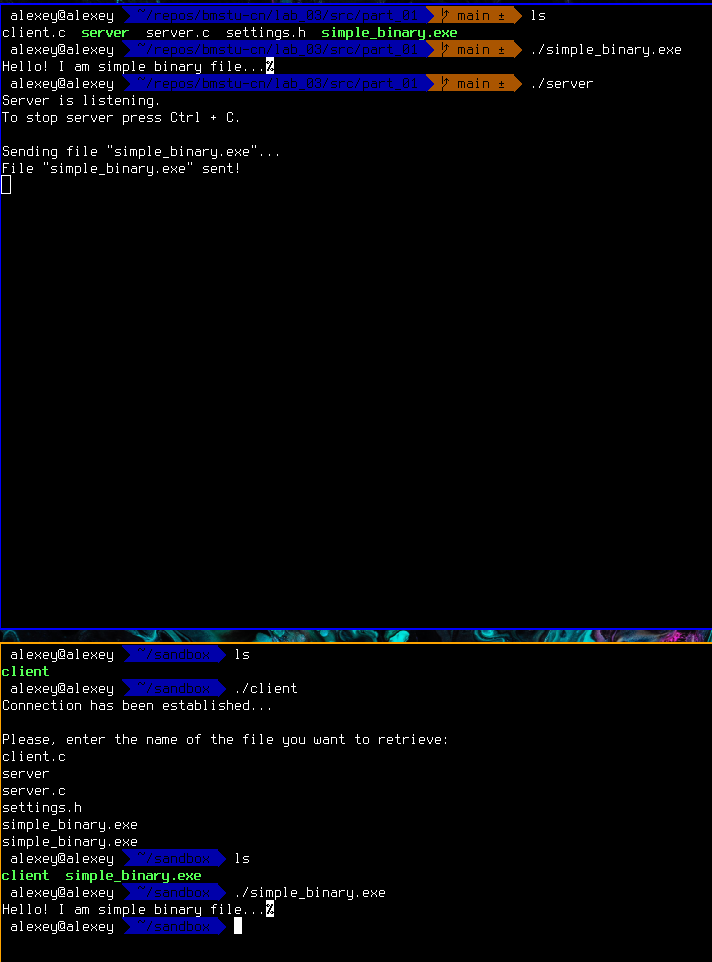
\includegraphics[scale=0.6]{img/prog_01.png}
	\end{center}
	\caption{Результат работы первой программы -- передача бинарного файла от сервера клиенту}
	\label{fig:prog_01}
\end{figure}

\subsection*{Часть 2}

\begin{figure}[H]
	\begin{center}
		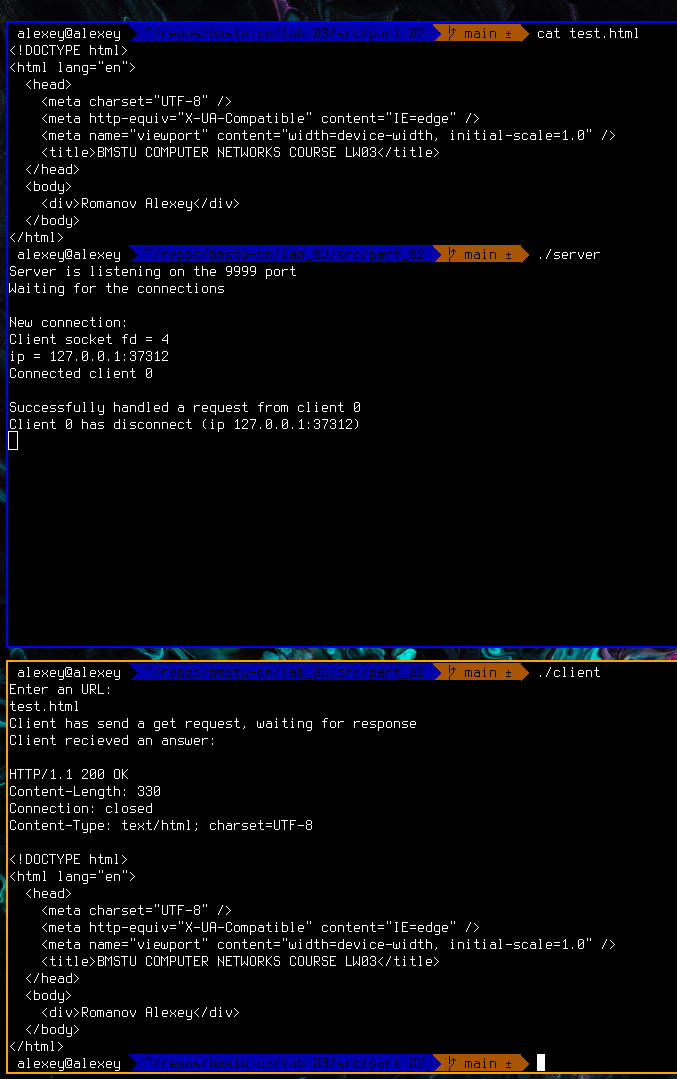
\includegraphics[scale=0.55]{img/prog_02_01.png}
	\end{center}
	\caption{Результат работы второй программы -- успешный GET-запрос}
	\label{fig:prog_02_01}
\end{figure}

\begin{figure}[H]
	\begin{center}
		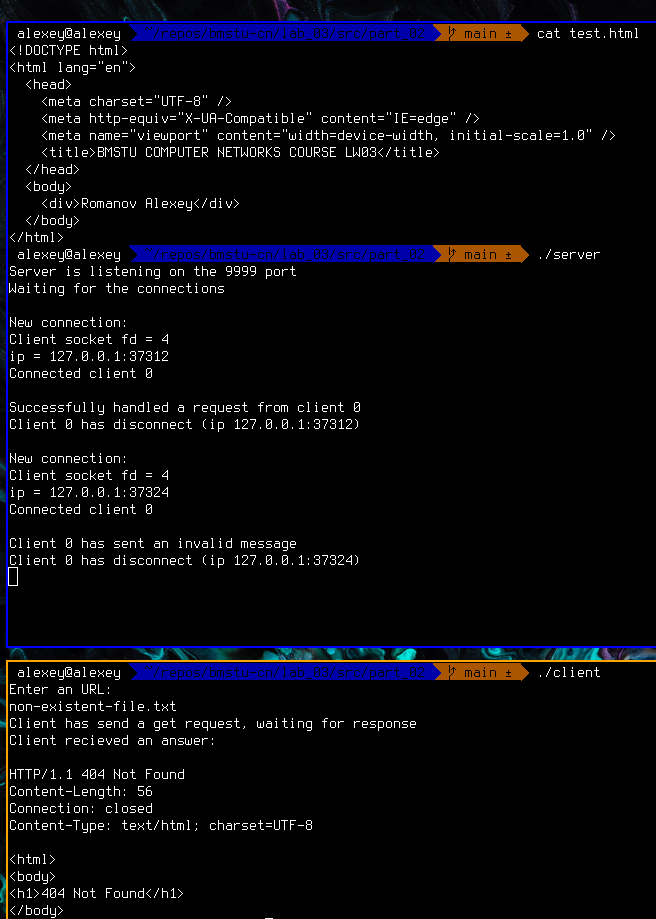
\includegraphics[scale=0.6]{img/prog_02_02.png}
	\end{center}
	\caption{Результат работы второй программы -- неуспешный GET-запрос (404)}
	\label{fig:prog_02_02}
\end{figure}

\begin{figure}[H]
	\begin{center}
		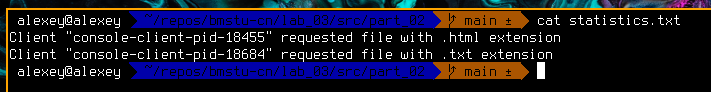
\includegraphics[scale=0.6]{img/prog_02_03.png}
	\end{center}
	\caption{Результат работы второй программы (доп. задание) -- логирование расширенией запрашиваемых клиентами файлов}
	\label{fig:prog_02_03}
\end{figure}

Исходный код программного обеспечения приложен (в архиве) к отчёту.

\bibliographystyle{utf8gost705u}
\bibliography{51-biblio}
	
\end{document}
